\documentclass[a4paper,12pt]{article}

% Packages
\usepackage[utf8]{inputenc}   % For UTF-8 encoding
\usepackage{amsmath}          % For advanced math formatting
\usepackage{amssymb}          % For additional math symbols
\usepackage{geometry}         % For adjusting margins
\geometry{margin=1in}

\usepackage{graphicx}
\usepackage{hyperref}
\usepackage{booktabs}
\usepackage{placeins}  % Add this in your preamble


% Document Settings
\setlength{\parindent}{0pt}   % No paragraph indentation
\setlength{\parskip}{1em}     % Add space between paragraphs


\title{Neural implicit representation of fixed topology under linear elastic deformation}
\author{François Pagé}
\date{}

\begin{document}
\maketitle
\begin{abstract}
	\centering
	This work presents a dynamic simulation of the Stanford Bunny undergoing small linear elastic deformation. Using the family of shapes generated by the simulation, we compute the signed distance function (SDF) at various points. A range of machine learning models with varying depths, widths, and training strategies are employed to predict SDF values. Our results provide insights into the minimum model size necessary for accurately capturing such dynamic deformations using deep learning techniques.
\end{abstract}

\newpage

\section*{Introduction and Related Works}
Even with modern hardware, real-time physics simulations remains computationally expensive. To remedy this, methods such as model reductions were used \cite{treuille2006model}, allowing their implementation in interactive mediums such as video games and medical simulations \cite{vanneste2020needle}.

Recently, mixed physics and neural networks based approach have shown a lot of premise after the success of \cite{deepsdf}. Furthermore, the speed improvement shown in \cite{neural_lod} further cemented their potentials. As such, this paper aims to recreate an neural network model of physics simulation on the Stanford bunny using signed distance functions (SDF) to implicitly represent the time evolution of the shape.

SDF are critical to this paper and it's inspirations and will therefore be explained first:
An SDF is a scalar field describing the distance from a point in space to the closest point on the surface of a domain (in this case the bunny's mesh). For points inside the domain, the result is negated.

To create a family of shape, the forward Euler implementation of the Galerkin method was used. The Galerkin method is a type of numerical technique for solving PDEs over a finite element domain.

Once the simulation is complete, a global enlarged bounding box is calculated, inside of which a set of points are generated. The SDF is calculated at those points for all shapes. These SDF values are then used to train a K=1-nearest neighbor (KNN-1) model and two multi-layer perceptrons (MLPs). The Mesh Encoder learns latent representations for the shapes, while the SDF Calculator predicts the SDF values for sampled query points depending on the latent vector. Finally, the Marching Cubes algorithm reconstructs the deformed shapes from the predicted SDF values.

\section*{Method}

\subsection*{1. Obtaining the mesh}

We use the Stanford Bunny mesh available from the Stanford Graphics Lab. \cite{stanford_bunny}.

The original \texttt{.obj} file is converted into a \texttt{.mesh} format using TetWild \cite{tetwild}. To prepare the mesh for our simulations, we apply the following transformations:

\begin{enumerate}
	\item All points are shifted downward by \( dz = 0.007 \).
	\item Set the minimum of x to 0 (Optional)
	\item Set the center in y to 0 (Optional)
	\item The mesh is not normalized to preserve its original proportions.
\end{enumerate}

This ensures all points at the bottom of its foot are bellow $z=0$.

To help the reader understand the scale of the mesh, the post-transformation bounding box is given:

\begin{table}[h!]
	\centering
	\begin{tabular}{@{}lll@{}}
		\toprule
		Coordinate & Minimum (m) & Maximum (m) \\ \midrule
		\(x\)      & 0.0         & 0.1551      \\
		\(y\)      & -0.0602     & 0.0602      \\
		\(z\)      & -0.0070     & 0.1472      \\ \bottomrule
	\end{tabular}
	\caption{Bounding box dimensions of the transformed Stanford Bunny mesh, in meters. }
\end{table}

\begin{figure}[h!]
	\centering
	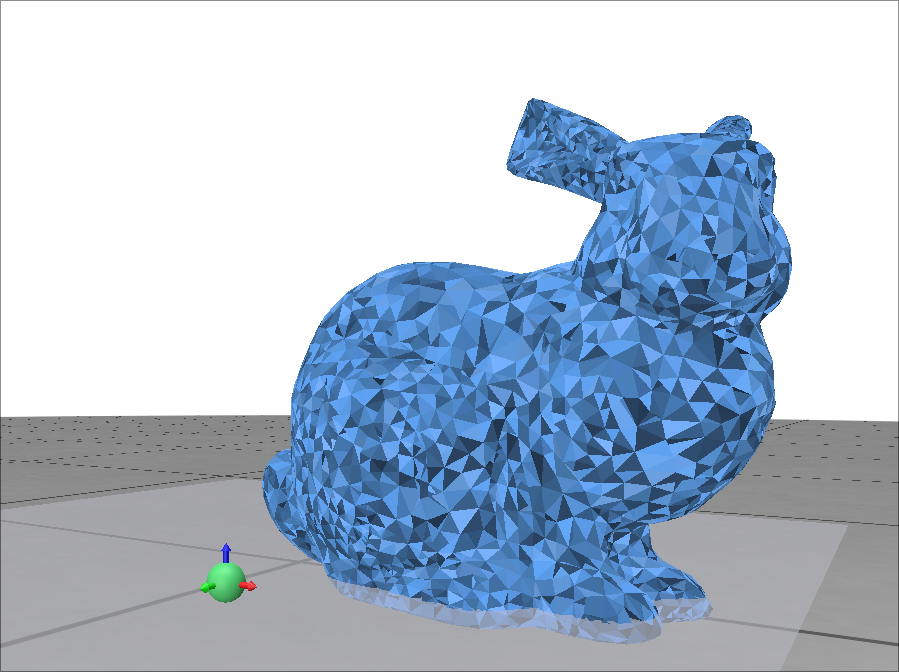
\includegraphics[width=0.8\textwidth]{proj/1-load-transform-bunny.png}
	\caption{Transformation of the Stanford Bunny during preprocessing, and the z=0 plane, bellow which the boundary points are fixed. }
	\label{fig:transform-bunny}
\end{figure}

\newpage
\subsection*{2. Physics simulation using the FEM method}
The family of curves is obtained by doing a dynamic physics simulation of linear elastic deformation of the stanford bunny being poked by a finger centered at $x_f$. This simulation is carried out using the Forward Euler method within the framework of the Galerkin method.

To represent the interaction between the finger and the bunny, we apply a constant pressure $p$ on the contact region. This region, denoted by $\Gamma$, is approximated as:

\[
	\Gamma = \{ x \in \partial \Omega \mid \|x - x_f\| \leq R \}.
\]
This generate a contact area $A \approx \pi R^2$ if the finger is near a low curvature point.

To ensure deformation rather then rigid body movement, we fix the bunny's foot to the floor by setting $u = 0$ on all boundary points with $ z \leq 0$
\newpage
With this setup, our goal is to solve the displacement vector field \( u(X, t) \) over the domain of the initial reference mesh \( \Omega \).

To achieve this, we begin by deriving the bilinear formulation from the strong form of the governing differential equations.

$$ \rho \frac{\partial ^2 u}{\partial t^2} - \nabla \cdot \sigma(u) = f$$
Applying time discretisation for the forward Euler's method, we obtain:
$$ \rho \frac{u_t^{n+1} - u_t^n}{\Delta t} - \nabla \cdot \sigma(u_n) = f$$
$$ \rho u_t^{n+1} - \rho u_t^n - \Delta t\nabla \cdot \sigma = \Delta t f$$
$$ \rho u_t^{n+1} = \Delta t f + \rho u_t^n - \Delta t\nabla \cdot \sigma (u_n)$$

We aim solve for $u_t^{n+1}$ using the Garlerkin's method, where the rest is seen as constant. The weak form is derived as follows:

% Multiply by a test function and integrate over the domain
\[
	\int_\Omega \rho u_t^{n+1} v \, d\Omega = \int_\Omega \Delta t f v \, d\Omega + \int_\Omega \rho u_t^n v \, d\Omega - \int_\Omega \Delta t (\nabla \cdot \sigma(u_n)) v \, d\Omega.
\]

% Apply the divergence theorem to the stress term
\[
	\int_\Omega (\nabla \cdot \sigma(u_n)) v \, d\Omega = \int_{\partial \Omega} (\sigma(u_n) \cdot n) v \, dS - \int_\Omega \sigma(u_n) : \nabla v \, d\Omega,
\]

% Substitute the divergence term back into the equation
\[
	\int_\Omega \rho u_t^{n+1} v \, d\Omega = \int_\Omega \Delta t f v \, d\Omega + \int_\Omega \rho u_t^n v \, d\Omega - \Delta t \left( \int_{\partial \Omega} (\sigma(u_n) \cdot n) v \, dS - \int_\Omega \sigma(u_n) : \nabla v \, d\Omega \right).
\]

% Boundary conditions: applied pressure term
\[
	\int_{\partial \Omega} (\sigma(u_n) \cdot n) v \, dS = \int_{\partial \Omega} p H v \, dS,
\]

The step function \( H \) is defined as:

\[
	H(x) =
	\begin{cases}
		1, & x \in \Gamma,    \\
		0, & x \notin \Gamma.
	\end{cases}
\]

This give the following weak form
\[
	\int_\Omega \rho u_t^{n+1} v \, d\Omega + \Delta t \int_\Omega \sigma(u_n) : \nabla v \, d\Omega = \int_\Omega \Delta t f v \, d\Omega + \int_\Omega \rho u_t^n v \, d\Omega + \Delta t \int_{\partial \Omega} p H v \, dS.
\]
\newpage
From which, we can get the bilinear and linear forms to solve with the galerkin method of Fenics-Dolfinx. \cite{dolfinx}

% Expanded final weak form
\[
	\int_\Omega \rho u_t^{n+1} v \, d\Omega = \int_\Omega \Delta t f v \, d\Omega + \int_\Omega \rho u_t^n v \, d\Omega + \Delta t \int_{\partial \Omega} p H v \, dS - \Delta t \int_\Omega \sigma(u_n) : \nabla v \, d\Omega.
\]

Under small linear elastic deformations: $\epsilon(v) = \nabla v$. Hence, we obtain
% Final weak form
\[
	a(u_t^{n+1}, v) = L(v),
\]

% Define bilinear and linear forms
% Bilinear form
\[
	a(u_t^{n+1}, v) = \int_\Omega \rho u_t^{n+1} v \, d\Omega.
\]

% Simplified linear form
\[
	L(v) = \int_\Omega \Delta t f v \, d\Omega + \int_\Omega \rho u_t^n v \, d\Omega + \Delta t \int_{\partial \Omega} p H v \, dS - \Delta t \int_\Omega \sigma(u_n) : \epsilon(v) \, d\Omega.
\]

The pseudo-code for the simulation can be expressed as follows:
\[
	t \gets t + \Delta t
\]
\[
	u_t^{n+1} = G(u^n, u_t^n)
\]
\[
	u^{n+1} = u^n + u_t^{n+1}  \Delta t
\]
\[
	n \gets n + 1
\]

\newpage

To obtain a visible deformation, we used the following material properties and parameters:

- Young's modulus: \( E = 5 \times 10^3 \, \text{Pa} \),
- Poisson's ratio: \( \nu = 0.40 \),
- Density: \( \rho = 1 \, \text{kg/m}^3 \).
- External Force Field: $f=0$

The region where the pressure is applied is defined as from the sphere:
- Radius: \( R = 0.003 \, \text{m} \),
- Pressure: \( p = 4000 \, \text{Pa} \).

To compute the Lamé parameters, we use the following relationships:

\[
	\mu = \frac{E}{2(1 + \nu)},
\]

\[
	\lambda = \frac{E \nu}{(1 + \nu)(1 - 2\nu)}.
\]

Substituting the given values:

\[
	\mu = \frac{5000}{2(1 + 0.40)} = \frac{5000}{2 \times 1.4} = \frac{5000}{2.8} \approx 1785.71 \, \text{Pa}.
\]

\[
	\lambda = \frac{5000 \times 0.40}{(1 + 0.40)(1 - 2 \times 0.40)} = \frac{2000}{1.4 \times 0.2} = \frac{2000}{0.28} \approx 7142.86 \, \text{Pa}.
\]

Thus, the Lamé parameters are:

\[
	\mu \approx 1785.71 \, \text{Pa}, \quad \lambda \approx 7142.86 \, \text{Pa}.
\]

These parameters are used in the stress-strain relationship for linear elasticity:

\[
	\sigma(u) = \lambda (\nabla \cdot u) I + 2 \mu \varepsilon(u),
\]

where:

\[
	\varepsilon(u) = \frac{1}{2} \left( \nabla u + (\nabla u)^T \right).
\]

We chose a finger position on the face of the bunny, causing the head to tilt backward.

\newpage
To ensure the results of the PDEs remain stable and do not diverge, it is essential to choose an appropriate time step \( \Delta t \).

The Courant time step limit, which provides a stability criterion for explicit time integration, is given by:

\[
	\Delta t_{\text{CFL}} \leq \frac{h}{c},
\]

where \( h \) represents the characteristic element size, determined as the smallest edge in the mesh, and \( c \) is the speed of sound in the material. The speed of sound is defined as:

\[
	c = \sqrt{\frac{\lambda + 2\mu}{\rho}}.
\]

By substituting the expressions for \( c \) and \( h \), the Courant time step limit becomes:

\[
	\Delta t_{\text{CFL}} = \frac{h}{\sqrt{\frac{\lambda + 2\mu}{\rho}}} = 3.45 \cdot 10 ^{-6}s
\]
Hence, we chose $\Delta t = 1.0\cdot10^{-6}s$
We run the simulation for 0.01 seconds, and save it's state to a file every 100 itterations.

Hence, we obtain 101 shapes.

\begin{figure}[h!]
	\centering
	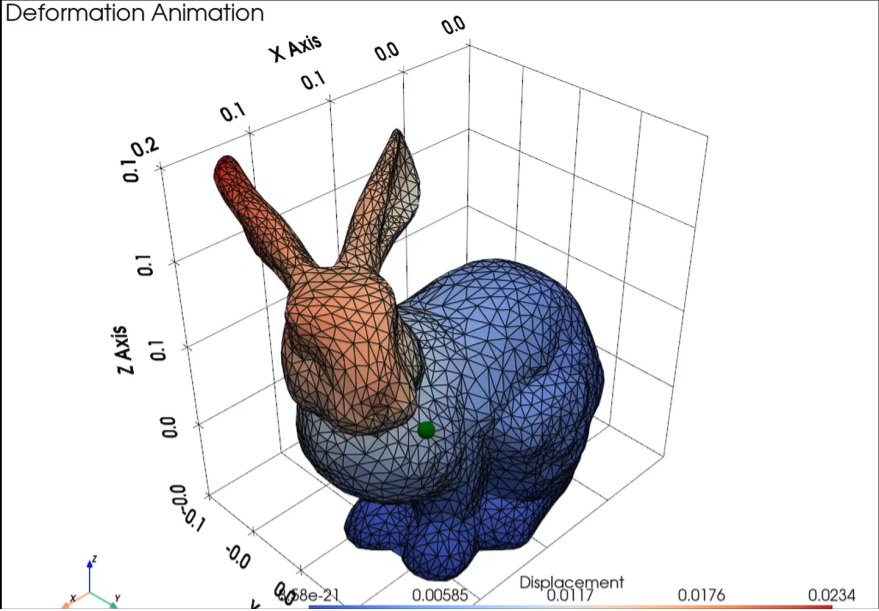
\includegraphics[width=0.8\textwidth]{proj/2-deformation-animation.png}
	\caption{Last frame of the physics simulation animation with the finger as a sphere to show the displacements. The finger initially touched the nose. }
	\label{fig:physics-animation-bunny}
\end{figure}

\subsection*{3. SDF Ground Truth Computation}

For each shape, we calculate its bounding box and then compute an enlarged bounding box with the same center but dimensions scaled by a factor of 1.5. The largest bounding box across all shapes is retained as the reference bounding box.

To ensure accurate sampling, a distribution of points was designed to place more weight on the bunny's head and ears (regions with high \( z \)-values), where movement and detail are more pronounced. A total of \( 1,000,000 \) ground truth training points were generated and shared across all shapes. This shared approach was adopted after observing no significant differences compared to using distinct point sets for each shape, owing to the high density of the sampled points.

The \( x \) and \( y \) coordinates are sampled uniformly within the enlarged bounding box, while the \( z \)-coordinate is sampled using the following formula:

\[
	P(z) \propto a(z - z_{\text{min}})^n + b,
\]

where:
\begin{itemize}
	\item \( n = 0.5 \),
	\item \( b = 0.001 \),
	\item \( a \) is a normalization constant ensuring the distribution sums to 1.
\end{itemize}

This produces the \( z \)-value distribution shown in the appendix (Figure~\ref{fig:original-points-xyz}).

These points are then filtered using a weighting function to prioritize points near the \( \text{SDF} = 0 \) isosurface. Additionally, since the bunny's volume is much smaller than the volume of the enlarged bounding box (volume ratio: 0.26), a weight is applied to increase the number of points inside the bunny.

The weighting function is defined as:

\[
	w \cdot (1 + |\text{SDF}|)^n,
\]

here:
\begin{itemize}
	\item \( w = 0.8 \) if \( \text{SDF} > 0 \), indicating points outside the object,
	\item \( w = 3 \) if \( \text{SDF} < 0 \), emphasizing points inside the object,
	\item \( n = 10 \), which controls the weight decay with distance from the surface.
\end{itemize}

Due to the random filtering process, each family of shapes produces slightly different numbers of points. To maintain consistency, we use the minimum number of points across all shapes. After filtering, we have \( 389,992 \) points, with the corresponding SDF distribution shown in Figure~\ref{fig:sdf-hist-filtered}.

\begin{figure}[h!]
	\centering
	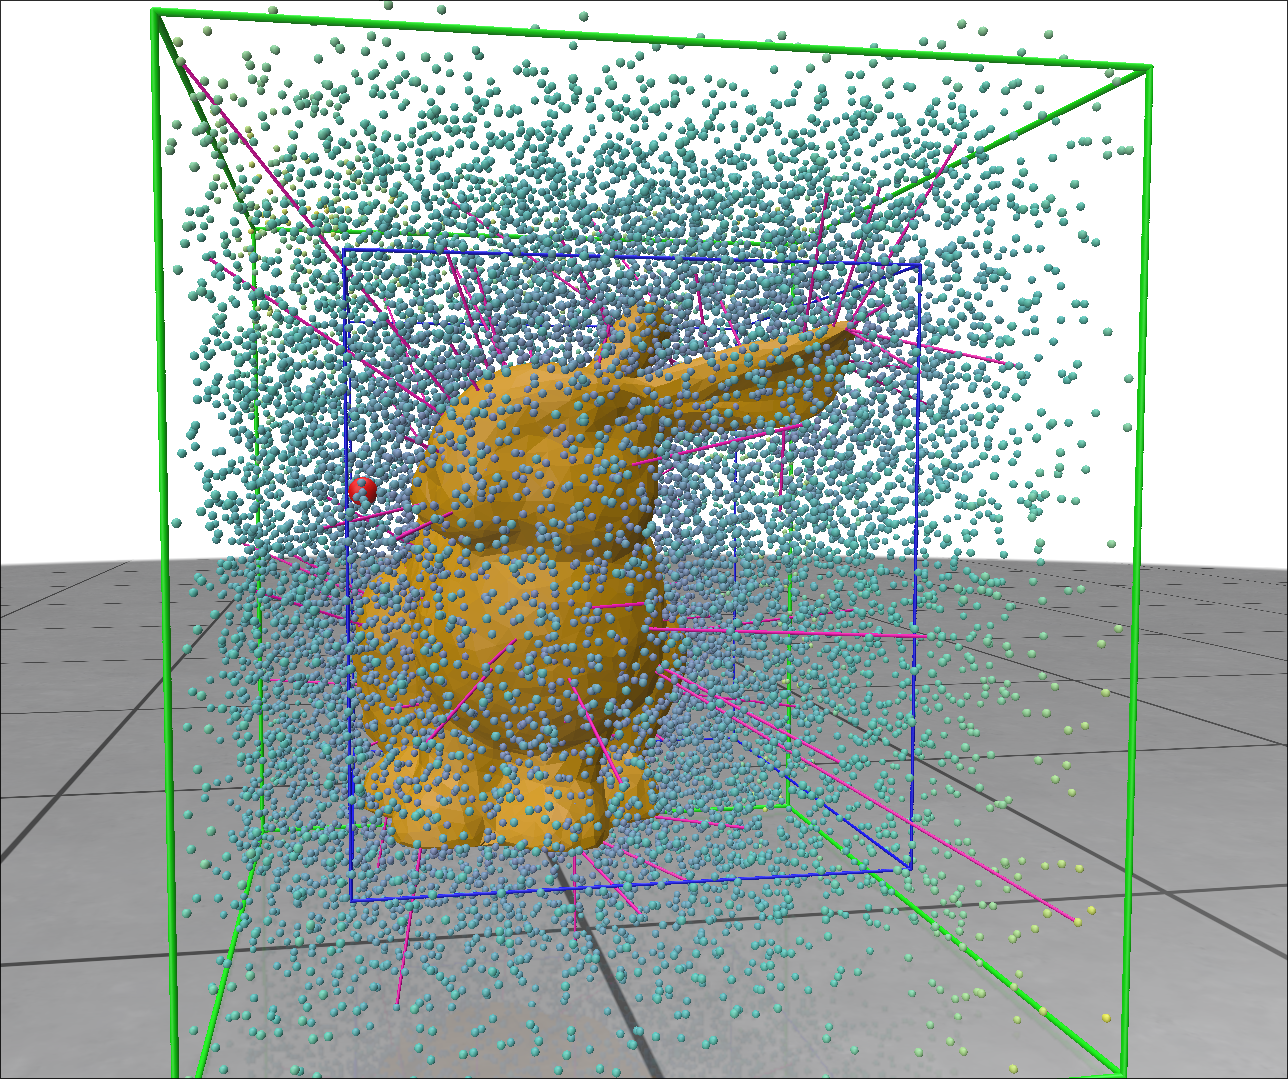
\includegraphics[width=0.8\textwidth]{proj/5-bbox-sdf-bunny.png}
	\caption{Visualization of the last frame showing the Stanford Bunny with the finger, the bounding boxes (green and purple), the first 10,000 SDF points colormapped by their values, and 100 lines connecting the points to their closest locations on the surface.}

	\label{fig:sdf-bbox}
\end{figure}

\subsection*{4. Machine Learning Framework}

The computation is divided into two neural networks: a \textbf{Mesh Encoder}, which outputs a 128-dimensional latent vector, and an \textbf{SDF Calculator}, which takes the latent vector and a point as input. Each shape is treated as a single batch during training.

The \textbf{Mesh encoder} started with an initial learning rate of 0.0075 and the \textbf{SDF Calculator} with 0.005
\subsubsection*{Mesh Encoder}
The Mesh Encoder is a Multi-Layer Perceptron (MLP) that processes the \( 10,338 \) vertices of the surface mesh. It consists of four layers with the following dimensions:

\[
	\text{input\_dim} \ (10,338) \rightarrow 256 \rightarrow 256 \rightarrow 128 \rightarrow \text{latent\_dim} \ (128).
\]

The mapping function of the Mesh Encoder is:

\[
	M(P_i) = z_i
\]

where:
\begin{itemize}
	\item \( P_i \) is the point cloud of the \( i \)-th shape's boundary with a fixed topology (i.e., the vertex positions).
	\item \( z_i \) is the latent vector encoding of the \( i \)-th shape.
\end{itemize}

\subsubsection*{SDF Calculator}
The SDF Calculator is another MLP that takes as input the concatenation of the latent vector and a 3D point. Its architecture is as follows:

\[
	(\text{latent\_dim} \ (128) + 3) \rightarrow 256 \rightarrow 256 \rightarrow 128 \rightarrow 1.
\]

The SDF function is defined as:

\[
	S(z_i, X) = d
\]

where:
\begin{itemize}
	\item \( z_i \) is the latent vector encoding of the \( i \)-th shape.
	\item \( X = (x, y, z) \) is a 3D point.
	\item \( d \) is the signed distance from \( X \) to the boundary of the \( i \)-th shape.
\end{itemize}

For both networks:
\begin{itemize}
	\item The first three layers use the \textbf{ReLU} activation function.
	\item The output layers have \textbf{no activation function}.
\end{itemize}

\subsubsection*{Schedulers}
Two learning rate schedulers are employed during training:
\begin{enumerate}
	\item \textbf{Scheduler 1:} Active from epoch 3 to epoch 19 (inclusive). This scheduler is updated after every batch, with the following parameters:
	      \begin{itemize}
		      \item \textbf{Patience:} 30 steps,
		      \item \textbf{Factor:} 0.92 (multiplies the learning rate by 0.92).
	      \end{itemize}
	\item \textbf{Scheduler 2:} Active from epoch 20 onward. This scheduler is updated based on the average validation loss over the 101 shapes for the current epoch, with:
	      \begin{itemize}
		      \item \textbf{Patience:} 2 epochs,
		      \item \textbf{Factor:} 0.75.
	      \end{itemize}
\end{enumerate}

\subsubsection*{Training Procedure}
The training process is divided into two stages:
\begin{enumerate}
	\item \textbf{Ordered Training (Epochs 1-6):} During the first six epochs, the shapes are passed in increasing and then decreasing order to keep the variations between batches small.
	\item \textbf{Shuffled Training (Epoch 7 onward):} The shapes are passed in a random order to generalize the model to the entire dataset.
\end{enumerate}

\subsubsection*{Cyclic Training Strategy}
The training alternates between three modes to encourage the Mesh Encoder to learn distinct latent representations for different shapes:
\begin{itemize}
	\item \textbf{Both Networks Active:} For 7 epochs.
	\item \textbf{Mesh Encoder Only:} For 5 epochs.
	\item \textbf{SDF Calculator Only:} For 12 epochs.
\end{itemize}

During the experimentation and fine-tuning process, the strategies were implemented incrementally, as described above. Initially, simpler neural networks with a depth of 3 and widths of 128 (instead of 256) were tested. These models often converged to local maxima, resulting in blob-like reconstructions instead of accurate shapes. To address this, the neural network size was increased, and its hyperparameters were tuned to achieve the best possible results. Building on this foundation, additional strategies were subsequently introduced, with each layer of experimentation refined through further parameter tuning. While no single strategy yielded a perfect result, combining these approaches provided insights into improving reconstruction quality.

\begin{quote}
	\textbf{Note:} In the latest model, the cycling order has been generalized. Allowing any fixed order. Furthermore, the length of each cycle has been
	generalized, using a function based on how many time this cycle has occured, and what's the current ocurrance number with L(n) > 1.
	Furthermore, the latent vector encoder gives a 32 dimensional latent vector, rather then 128.
\end{quote}

\subsubsection*{Loss Calculation and Latent vector difference enforcement}
To force two different shape to not be encoded to the same latent vector, the cosine similarity between latent vector where compared and penalized.

First, we take the shape from two different time index. Since we have time index shuffling starting from some epoch, we must not equally penalize
the cosine similarity of the two latent vectors, as the difference should increase over time. We must also penalize sdf difference at the query points.

As, such, we would want something with behavior akin to $\frac{1 - C}{\Delta_t}$. Multiple hyper parametric function where tested and the following
where chosen.

The total loss function is defined as:

\begin{equation}
	L = \alpha_{\text{sdf}} \cdot L_{\text{sdf}} + \alpha_{\text{latent}} \cdot L_{\text{latent}}
\end{equation}

where the signed distance function (SDF) loss is computed as:

\begin{equation}
	L_{\text{sdf}} = \frac{L_{\text{sdf},1} + L_{\text{sdf},2}}{2}
\end{equation}

The two SDF Loss where calculated over a time index (A single bunny, 1 frame), using Mean Square Loss.

In particular, each individual SDF loss term is computed as:

\begin{equation}
	L_{\text{sdf}, i} = \frac{1}{|Q_i|} \sum_{X \in Q_i} \left( \text{SDF}(z_i, X) - \text{SDF}_{i, \text{Ground}}(X) \right)^2
\end{equation}

where:
\begin{itemize}
	\item \( L_{\text{sdf}, i} \) is the mean squared error for latent vector \( z_i \) at time index \( i \).
	\item \( Q_i \) is the set of query points for the \( i \)-th time index.
	\item \( |Q_i| \) represents the number of query points in \( Q_i \).
	\item \( \text{SDF}(z_i, X) \) is the predicted signed distance function value at query point \( X \) using latent vector \( z_i \).
	\item \( \text{SDF}_{i, \text{Ground}}(X) \) is the ground truth signed distance function at \( X \).
\end{itemize}

and the latent loss is given by:

\begin{equation}
	L_{\text{latent}} = \frac{1}{f_{\text{td}}(t)} \cdot \frac{1}{\sqrt{10^{-6} + |1 - C|}}
\end{equation}

where:

\begin{equation}
	C = \frac{\mathbf{z}_1 \cdot \mathbf{z}_2}{\|\mathbf{z}_1\| \|\mathbf{z}_2\|}
\end{equation}

is the cosine similarity between latent vectors \( \mathbf{z}_1 \) and \( \mathbf{z}_2 \), and

\begin{equation}
	f_{\text{td}}(t) = \sqrt{t^2 + 5t + 10}
\end{equation}

is a time-dependent scaling function, with:

\begin{equation}
	t = |t_2 - t_1|
\end{equation}

representing the absolute difference in both time index.

The functions \( \alpha_{\text{latent}} \) and \( \alpha_{\text{sdf}} \) are defined as follows:

\begin{equation}
	\alpha_{\text{latent}}(e) =
	\begin{cases}
		\frac{0.0005}{(e + 1)^{1.4}}, & \text{if } e < 200 \\
		0,                            & \text{otherwise}
	\end{cases}
\end{equation}

The function \( \alpha_{\text{sdf}} \) always returns:

\begin{equation}
	\alpha_{\text{sdf}}(e) = 1.
\end{equation}

where \( e \) represents the training epoch.

\subsubsection*{Shape Reconstructions}

Shape reconstructions were performed using the Marching Cubes algorithm. A \( 100 \times 100 \times 100 \) grid of SDF values was computed over the enlarged bounding box of each shape, and the \( \text{SDF} = 0 \) isosurface was extracted to recreate the shapes.

\begin{figure}[h!]
	\centering
	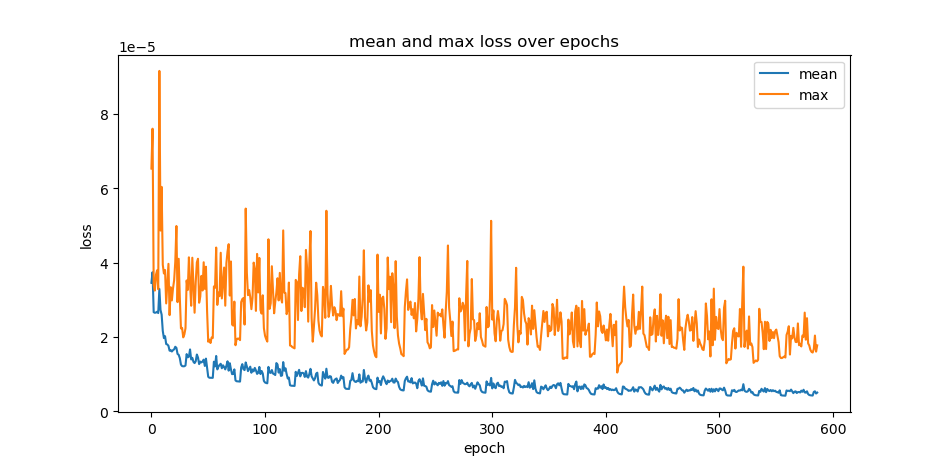
\includegraphics[width=0.8\textwidth]{proj/7-loss}
	\caption{Mean and Max Validation loss of batches over epochs}
	\label{fig:validation_loss_tracking}
\end{figure}

\newpage
\pagebreak
\section*{Results}

For comparison against an ideal outcome, the raw SDF data was sent to a \( k\)-Nearest Neighbor (KNN-1) neural network. This network was used to recreate the animations based on the raw ground truth SDF values, providing a benchmark for assessing the quality of the neural network-generated results.

Below is a comparison between the reconstructed shapes from the trained networks and the KNN-1 benchmark:

\begin{figure}[h!]
	\centering
	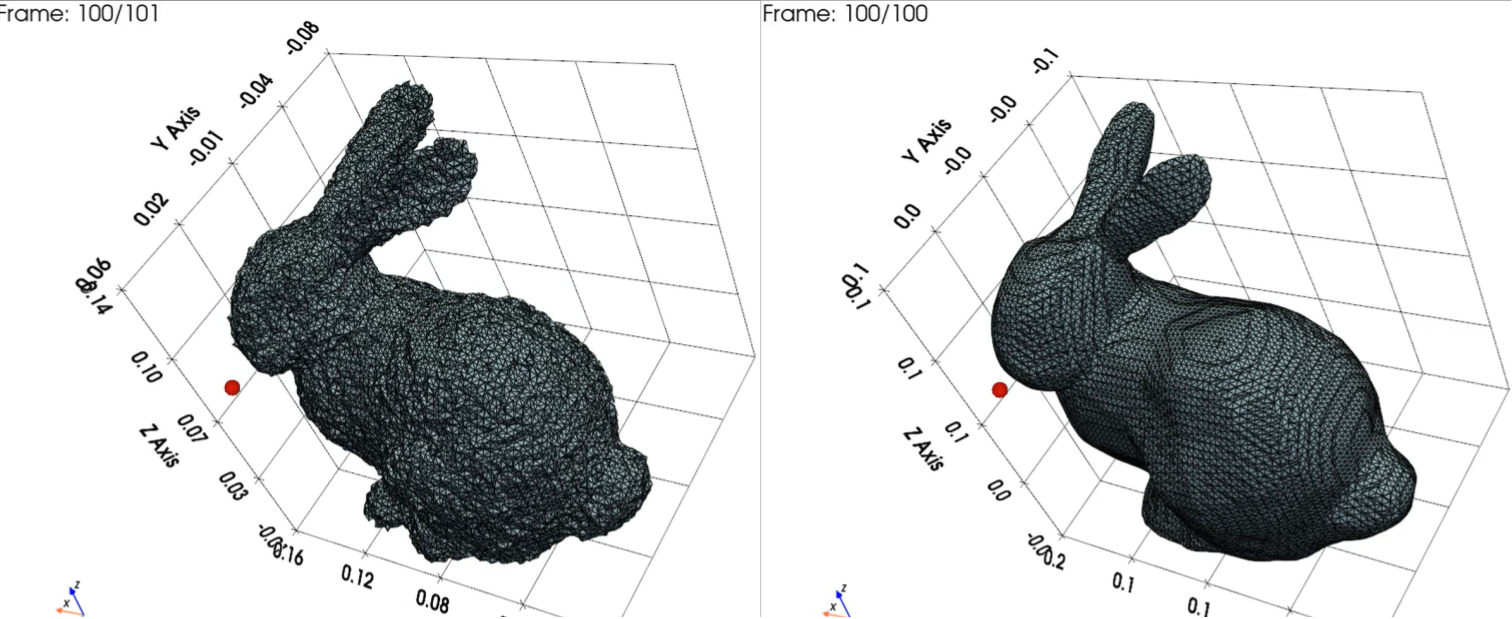
\includegraphics[width=0.8\textwidth]{proj/6-recreation-comparaison.png}
	\caption{Recreation of the last frame of the animation. KNN on the left, MLP on the Right. Epoch 592}
	\label{fig:recreation-comparaison}
\end{figure}

The latent vector did differ after adding the cosine similarity. Plots can be seen in the appendix

\newpage
\pagebreak

\section*{Conclusion}

The goal of encoding a family of shapes using an implicit neural network was achieved. However, the reconstructed shapes lacked detail. To address this, incorporating Fourier features before the mesh encoding could enable the neural network to capture higher-frequency data, leading to improved precision.

Beyond improving reconstruction accuracy, this framework can be extended to generalize across multiple physics simulations. By expanding the dataset with simulations that vary force positions and directions, we can construct a more comprehensive latent space representation of deformations. Once all shapes have been encoded, a secondary neural network can be trained to map force parameters—position, direction, and time—to a latent vector representation. This results in the structured transformation:

\[
	(\text{force position}, \text{force direction}, t) \rightarrow \text{latent vector} \rightarrow \text{SDF} \rightarrow \text{shape}.
\]

With this formulation, the neural network could predict deformations based on unseen force conditions. Furthermore, by integrating a Hamiltonian latent ODE neural network, we could establish a differential equation-based representation, enabling continuous, time-dependent deformations.

Finally, leveraging Neural Geometric Level of Detail (NGLoD) techniques could significantly enhance SDF computation speed and reconstruction efficiency. This improvement would make real-time applications of neural-augmented physics simulations more viable, bridging the gap between accuracy and computational feasibility.

\newpage
\pagebreak
\section*{Appendix}

\begin{figure}[h!]
	\centering
	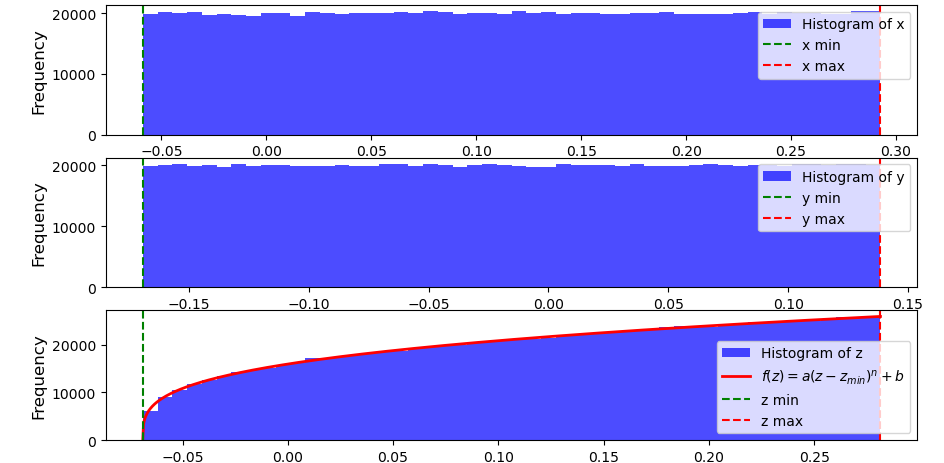
\includegraphics[width=0.8\textwidth]{proj/3-original-points.png}
	\caption{Histograms of the original points created before filtering}
	\label{fig:original-points-xyz}
\end{figure}

\begin{figure}[h!]
	\centering
	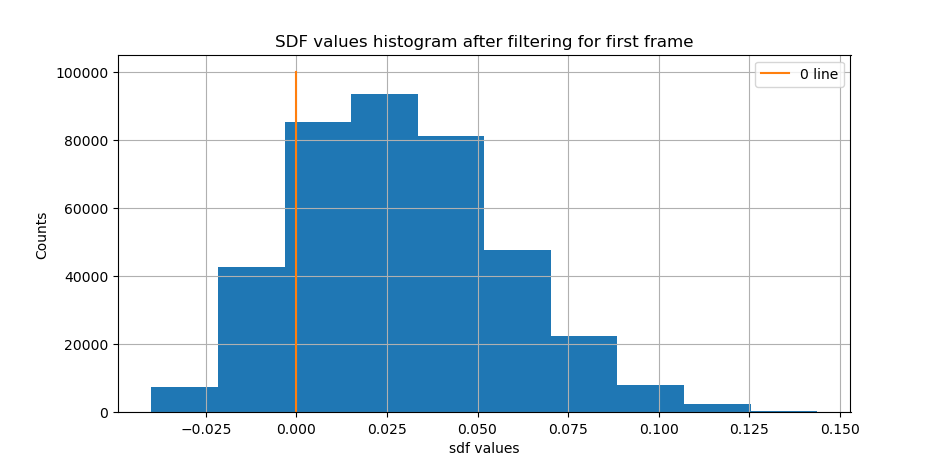
\includegraphics[width=0.8\textwidth]{proj/4-sdf-filtered.png}
	\caption{Histogram of the SDF values after filtering. (First frame of the animations)}
	\label{fig:sdf-hist-filtered}
\end{figure}

\begin{figure}[h!]
	\centering
	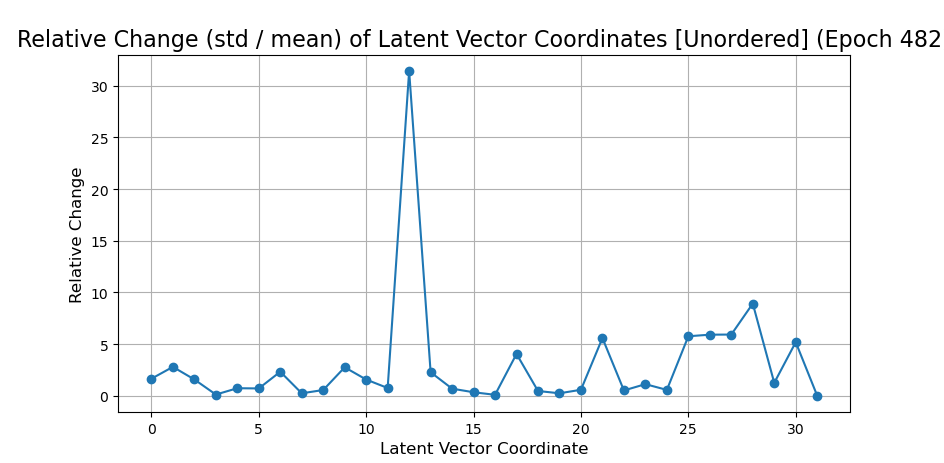
\includegraphics[width=0.8\textwidth]{./Latent Plots/Figure_1.png}
	\caption{Relative change of latent vector coordinates (Epoch 482)}
	\label{fig:relative-change-unordered}
\end{figure}

\begin{figure}[h!]
	\centering
	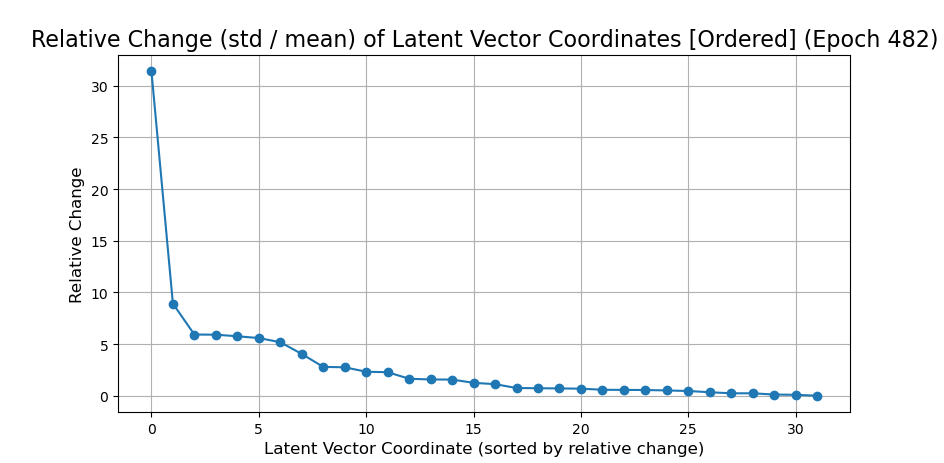
\includegraphics[width=0.8\textwidth]{./Latent Plots/Figure_2.png}
	\caption{Relative change of latent vector coordinates (Ordered) (Epoch 482)}
	\label{fig:relative-change-ordered}
\end{figure}

\begin{figure}[h!]
	\centering
	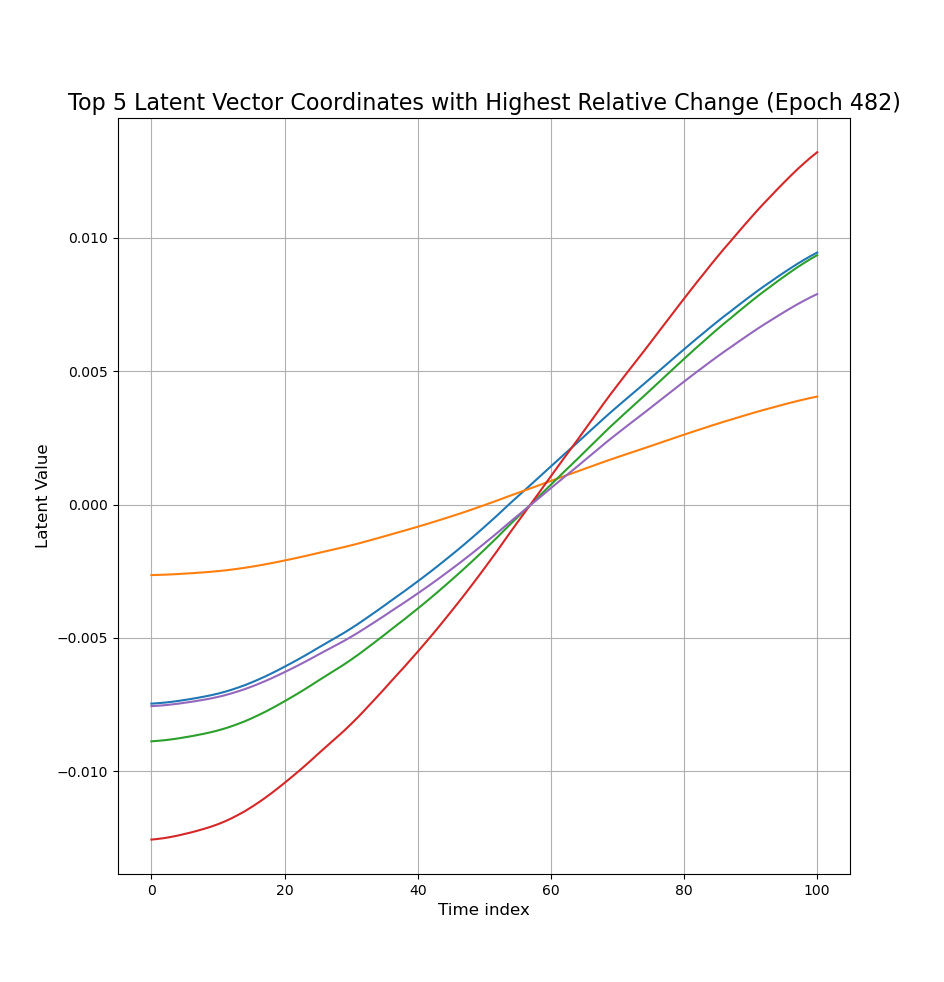
\includegraphics[width=0.8\textwidth]{./Latent Plots/Figure_3.png}
	\caption{Latent coordinates changes over times (Top 5 most changing), Epoch 482}
	\label{fig:latent-vector-top-5}
\end{figure}

\begin{figure}[h!]
	\centering
	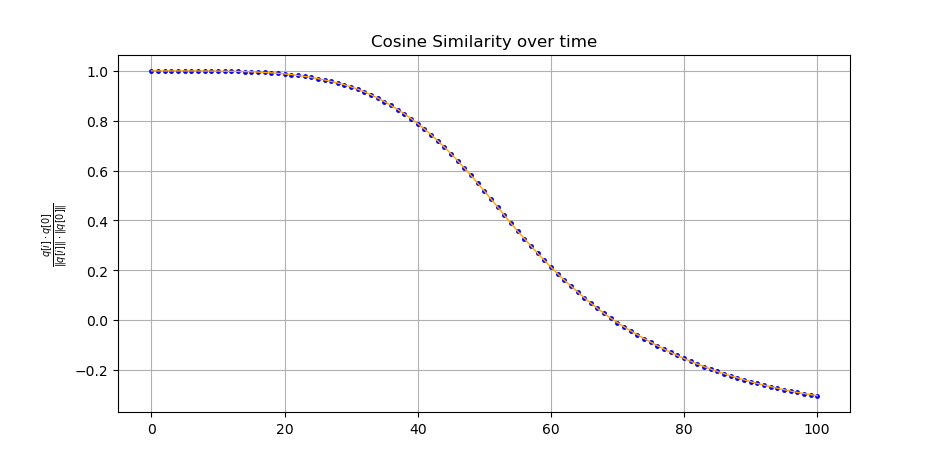
\includegraphics[width=0.8\textwidth]{./Latent Plots/Figure_4.png}
	\caption{Cosine Similarity over time of $z_i$ with $z_0$, epoch 482}
	\label{fig:cosine-similarity}
\end{figure}

\begin{quote}
	\textbf{Note:} Further work has been done since the last formal editing of this document, making it possible for there to be some inconsistencies
	inside of it. A complete consistency check is done after every major landmark.
\end{quote}

\FloatBarrier
\newpage
\pagebreak
\begin{thebibliography}{9}
	\bibitem{stanford_bunny}
	Stanford Graphics Lab, \emph{Stanford Bunny Mesh}, accessed from \href{https://graphics.stanford.edu/~mdfisher/Data/Meshes/bunny.obj}{https://graphics.stanford.edu/~mdfisher/Data/Meshes/bunny.obj}.

	\bibitem{tetwild}
	TetWild, \emph{Robust Tetrahedral Meshing}, available at \href{https://github.com/Yixin-Hu/TetWild}{https://github.com/Yixin-Hu/TetWild}.

	\bibitem{dolfinx}
	FEniCS Project, \emph{DOLFINx: A finite element computing platform}, available at \href{https://github.com/FEniCS/dolfinx}{https://github.com/FEniCS/dolfinx}.

	\bibitem{treuille2006model}
	Adrien Treuille, Andrew Lewis, and Zoran Popović.
	\emph{Model Reduction for Real-time Fluids}.
	ACM Transactions on Graphics (SIGGRAPH 2006), pages 826--834, 2006.

	\bibitem{vanneste2020needle}
	F{\'e}lix Vanneste, Claire Martin, Olivier Goury, Hadrien Courtecuisse, Erik Pernod, Stephane Cotin, and Christian Duriez.
	\emph{Towards realistic needle insertion training simulator using partitioned model order reduction}.
	In Proceedings of the 2020 Medical Image Computing and Computer-Assisted Intervention (MICCAI), 2020. Springer.

	\bibitem{deepsdf}
	Jeong Joon Park, Peter Florence, Julian Straub, Richard Newcombe, and Steven Lovegrove.
	\emph{DeepSDF: Learning Continuous Signed Distance Functions for Shape Representation}.
	In Proceedings of the IEEE Conference on Computer Vision and Pattern Recognition (CVPR), 2019

	\bibitem{neural_lod}
	Towaki Takikawa, Joey Litalien, Kangxue Yin, Karsten Kreis, Charles Loop, Derek Nowrouzezahrai, Alec Jacobson, Morgan McGuire, and Sanja Fidler.
	\emph{Neural Geometric Level of Detail: Real-time Rendering with Implicit 3D Shapes}.
	In Proceedings of the IEEE Conference on Computer Vision and Pattern Recognition (CVPR), 2021

\end{thebibliography}
\end{document}
